\documentclass[border=4pt]{standalone}
\usepackage{fontspec}
\setmainfont{DMSans9pt}[Path=../../fonts/, Extension=.ttf, UprightFont=*-Regular, BoldFont=*-Bold, ItalicFont=*-Italic, BoldItalicFont=*-BoldItalic]
\setsansfont{DMSans9pt}[Path=../../fonts/, Extension=.ttf, UprightFont=*-Regular, BoldFont=*-Bold, ItalicFont=*-Italic, BoldItalicFont=*-BoldItalic]
\usepackage{amsmath,amssymb,xcolor,adjustbox,pifont}
\usepackage{tikz}
\usetikzlibrary{arrows.meta,positioning,shapes.geometric,shapes.misc,fit,backgrounds,calc,decorations.pathreplacing,shadows}
\usepackage[edges]{forest}
\usepackage{pgfplots}
\pgfplotsset{compat=1.18}

%% ---------- colours and macros used throughout
\definecolor{cTwo}{HTML}{4C72B0}   % two-stage
\definecolor{cOne}{HTML}{DD8452}   % one-stage / YOLO
\definecolor{cDetr}{HTML}{55A868}  % DETR
\definecolor{cOvd}{HTML}{8172B3}   % open-vocabulary
\definecolor{cAgent}{HTML}{C44E52} % agentic
\definecolor{cEdge}{HTML}{937860}  % edge
\definecolor{cApp}{HTML}{DA8BC3}   % applications
\definecolor{cData}{HTML}{4C9BB0}  % data / metrics
\newcommand{\tleaf}[1]{\parbox{8.3cm}{\raggedright #1}}
\newcommand{\tmid}[1]{\parbox{2.9cm}{\raggedright #1}}
\newcommand{\tone}[1]{\parbox{2.3cm}{\raggedright #1}}
\newcommand{\cmark}{\ding{51}}
\newcommand{\xmark}{\ding{55}}
\newcommand{\pmark}{$\circ$}


\renewcommand{\cite}[1]{}
\providecommand{\ref}[1]{}
\renewcommand{\ref}[1]{}
\newcommand{\tbd}[1]{#1}
\begin{document}
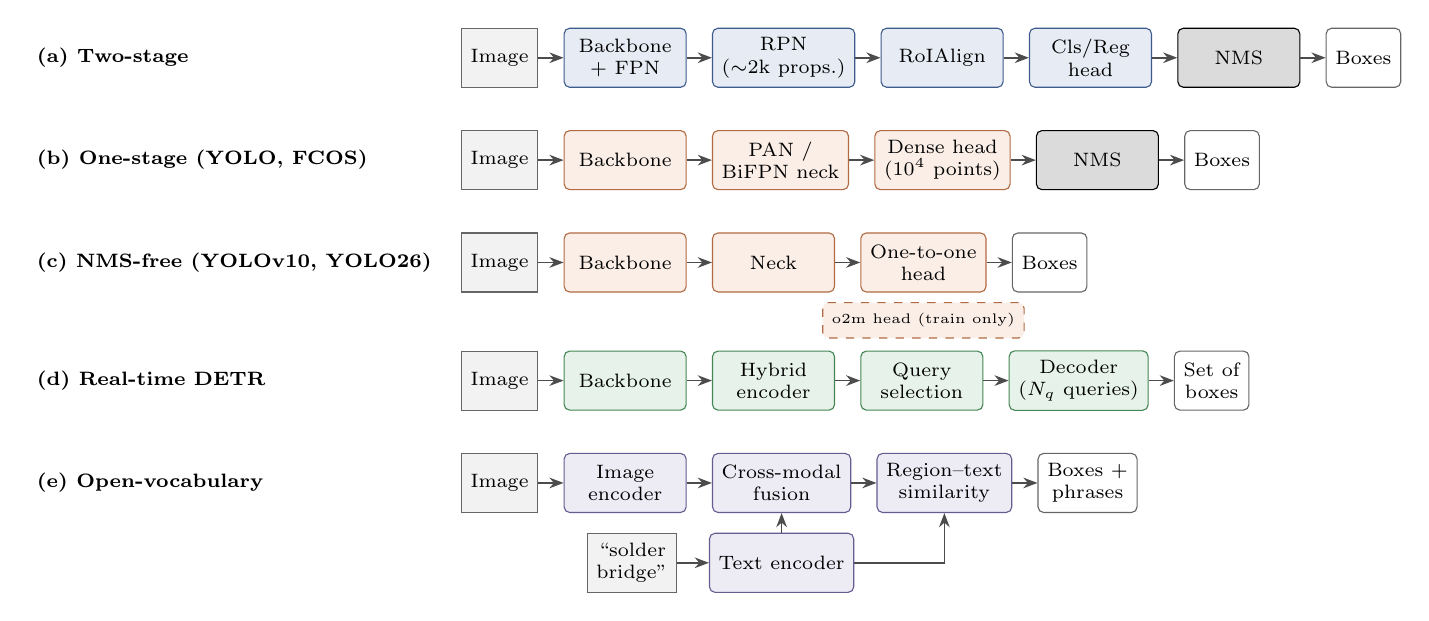
\begin{tikzpicture}[
  blk/.style={draw=#1!80!black, fill=#1!14, rounded corners=2pt, minimum height=0.75cm, minimum width=1.55cm, align=center, font=\scriptsize},
  img/.style={draw=black!60, fill=black!5, minimum width=0.9cm, minimum height=0.75cm, font=\scriptsize, align=center},
  outb/.style={draw=black!60, fill=white, rounded corners=2pt, minimum height=0.75cm, font=\scriptsize, align=center},
  lab/.style={font=\bfseries\scriptsize, anchor=west, align=left},
  arr/.style={-{Stealth[length=1.8mm]}, line width=0.6pt, black!70},
  node distance=0.32cm
]
% row 1: two-stage
\node[lab] (l1) at (0,0) {(a) Two-stage};
\node[img] (i1) at (6.0,0) {Image};
\node[blk=cTwo, right=of i1] (b1) {Backbone\\+ FPN};
\node[blk=cTwo, right=of b1] (r1) {RPN\\($\sim$2k props.)};
\node[blk=cTwo, right=of r1] (a1) {RoIAlign};
\node[blk=cTwo, right=of a1] (h1) {Cls/Reg\\head};
\node[blk=black, right=of h1] (n1) {NMS};
\node[outb, right=of n1] (o1) {Boxes};
\foreach \u/\v in {i1/b1,b1/r1,r1/a1,a1/h1,h1/n1,n1/o1} \draw[arr] (\u)--(\v);
% row 2: one-stage
\node[lab] (l2) at (0,-1.3) {(b) One-stage (YOLO, FCOS)};
\node[img] (i2) at (6.0,-1.3) {Image};
\node[blk=cOne, right=of i2] (b2) {Backbone};
\node[blk=cOne, right=of b2] (k2) {PAN /\\BiFPN neck};
\node[blk=cOne, right=of k2] (h2) {Dense head\\($10^4$ points)};
\node[blk=black, right=of h2] (n2) {NMS};
\node[outb, right=of n2] (o2) {Boxes};
\foreach \u/\v in {i2/b2,b2/k2,k2/h2,h2/n2,n2/o2} \draw[arr] (\u)--(\v);
% row 3: NMS-free one-stage
\node[lab] (l3) at (0,-2.6) {(c) NMS-free (YOLOv10, YOLO26)};
\node[img] (i3) at (6.0,-2.6) {Image};
\node[blk=cOne, right=of i3] (b3) {Backbone};
\node[blk=cOne, right=of b3] (k3) {Neck};
\node[blk=cOne, right=of k3] (h3) {One-to-one\\head};
\node[outb, right=of h3] (o3) {Boxes};
\node[blk=cOne, below=0.12cm of h3, dashed, font=\tiny, minimum height=0.45cm] (aux3) {o2m head (train only)};
\foreach \u/\v in {i3/b3,b3/k3,k3/h3,h3/o3} \draw[arr] (\u)--(\v);
% row 4: DETR
\node[lab] (l4) at (0,-4.1) {(d) Real-time DETR};
\node[img] (i4) at (6.0,-4.1) {Image};
\node[blk=cDetr, right=of i4] (b4) {Backbone};
\node[blk=cDetr, right=of b4] (e4) {Hybrid\\encoder};
\node[blk=cDetr, right=of e4] (q4) {Query\\selection};
\node[blk=cDetr, right=of q4] (d4) {Decoder\\($N_q$ queries)};
\node[outb, right=of d4] (o4) {Set of\\boxes};
\foreach \u/\v in {i4/b4,b4/e4,e4/q4,q4/d4,d4/o4} \draw[arr] (\u)--(\v);
% row 5: OVD
\node[lab] (l5) at (0,-5.4) {(e) Open-vocabulary};
\node[img] (i5) at (6.0,-5.4) {Image};
\node[blk=cOvd, right=of i5] (b5) {Image\\encoder};
\node[blk=cOvd, right=of b5] (f5) {Cross-modal\\fusion};
\node[blk=cOvd, right=of f5] (h5) {Region--text\\similarity};
\node[outb, right=of h5] (o5) {Boxes +\\phrases};
\node[blk=cOvd, below=0.25cm of f5] (t5) {Text encoder};
\node[img, left=0.4cm of t5] (p5) {``solder\\bridge''};
\draw[arr] (p5)--(t5); \draw[arr] (t5)--(f5); \draw[arr] (t5.east) -| (h5.south);
\foreach \u/\v in {i5/b5,b5/f5,f5/h5,h5/o5} \draw[arr] (\u)--(\v);
\end{tikzpicture}
\end{document}
